\documentclass[border=4pt]{standalone}
% Preámbulo común de las figuras. Cada figura es un documento standalone
% que se compila a SVG con scripts/build_figures.sh
\usepackage[utf8]{inputenc}
\usepackage{amsmath}
\usepackage{tikz}
\usepackage[american, siunitx]{circuitikz}
\usetikzlibrary{arrows.meta,calc,decorations.pathmorphing,patterns}
\tikzset{
  >={Stealth[length=2.2mm]},
  eje/.style={->, thin},
  hilo/.style={thick},
}
% Paleta común: tonos medios legibles sobre fondo claro
\definecolor{azul}{RGB}{31,94,168}
\definecolor{rojo}{RGB}{192,57,43}
\definecolor{verde}{RGB}{39,128,73}
\definecolor{naranja}{RGB}{211,120,30}
\definecolor{morado}{RGB}{125,60,152}

\begin{document}
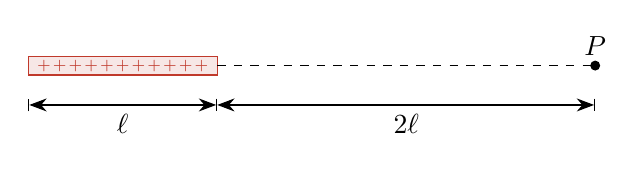
\begin{tikzpicture}[scale=1.0]
  \draw[rojo, fill=rojo!12] (0,-0.12) rectangle (2.4,0.12);
  \foreach \x in {0.2,0.4,...,2.2} \node[font=\tiny, rojo] at (\x,0) {$+$};
  \draw[dashed] (2.4,0) -- (7.2,0);
  \fill (7.2,0) circle (1.8pt) node[above]{$P$};
  \draw[|<->|] (0,-0.5) -- node[below]{$\ell$} (2.4,-0.5);
  \draw[<->|] (2.4,-0.5) -- node[below]{$2\ell$} (7.2,-0.5);
\end{tikzpicture}
\end{document}
